\documentclass[letterpaper,12pt]{article}
\usepackage{array}
\usepackage{threeparttable}
\usepackage{geometry}

\usepackage{natbib}

%\usepackage{jf} %always check the instruction of the package to see if it conflicts
\geometry{letterpaper,tmargin=1in,bmargin=1in,lmargin=1.25in,rmargin=1.25in}
\usepackage{fancyhdr,lastpage}
\pagestyle{fancy}
\lhead{}
\chead{}
\rhead{}
\lfoot{}
\cfoot{}
\rfoot{\footnotesize\textsl{Page \thepage\ of \pageref{LastPage}}}
\renewcommand\headrulewidth{0pt}
\renewcommand\footrulewidth{0pt}
\usepackage[format=hang,font=normalsize,labelfont=bf]{caption}
\usepackage{listings}
\lstset{frame=single,
  language=Python,
  showstringspaces=false,
  columns=flexible,
  basicstyle={\small\ttfamily},
  numbers=none,
  breaklines=true,
  breakatwhitespace=true
  tabsize=3
}
\usepackage{amsmath}
\usepackage{amssymb}
\usepackage{amsthm}
%\usepackage{harvard}
\usepackage{setspace}
\usepackage{float,color}
\usepackage[pdftex]{graphicx}
\usepackage{hyperref}
\hypersetup{colorlinks,linkcolor=red,urlcolor=blue,citecolor=blue}
\theoremstyle{definition}
\newtheorem{theorem}{Theorem}
\newtheorem{acknowledgement}[theorem]{Acknowledgement}
\newtheorem{algorithm}[theorem]{Algorithm}
\newtheorem{axiom}[theorem]{Axiom}
\newtheorem{case}[theorem]{Case}
\newtheorem{claim}[theorem]{Claim}
\newtheorem{conclusion}[theorem]{Conclusion}
\newtheorem{condition}[theorem]{Condition}
\newtheorem{conjecture}[theorem]{Conjecture}
\newtheorem{corollary}[theorem]{Corollary}
\newtheorem{criterion}[theorem]{Criterion}
\newtheorem{definition}[theorem]{Definition}
\newtheorem{derivation}{Derivation} % Number derivations on their own
\newtheorem{example}[theorem]{Example}
\newtheorem{exercise}[theorem]{Exercise}
\newtheorem{lemma}[theorem]{Lemma}
\newtheorem{notation}[theorem]{Notation}
\newtheorem{problem}[theorem]{Problem}
\newtheorem{proposition}{Proposition} % Number propositions on their own
\newtheorem{remark}[theorem]{Remark}
\newtheorem{solution}[theorem]{Solution}
\newtheorem{summary}[theorem]{Summary}
%\numberwithin{equation}{section}
%\bibliographystyle{aer}
\newcommand\ve{\varepsilon}
\newcommand\boldline{\arrayrulewidth{1pt}\hline}

\DeclareMathOperator*{\argmax}{arg\,max}

\usepackage{graphicx}
\graphicspath{ {c:/users/yafei/compecon_fall17/visualization} }

\title{Problem Set 8: General Equilibrium of Firm's Problem}
\author{Yafei Zhang \thanks{Yafei Zhang is from Finance department of USC, he can be reached at yafei.zhang@grad.moore.sc.edu.}}
\date{November 1 2017}

\begin{document}

\maketitle

\vspace{5mm}

\section{Introduction}

In this problem set, I will numerically solve out a general equilibrium problem for the firms with stochastic productivities and quadratic adjustment costs. This problem set is a joint work with Destan and Foteini. I was happy working together with them. We wrote the codes step by step and tried our best to make the codes as efficient as possible. The structure of this problem set is as follows. In section 2, I will briefly go through the model theoretically. Section 3 will explain the codes. Section 4 describes the equilibrium results.


\section{Firm's Problem}

The firm's problem can be summarized through the Bellman equation:
\begin{equation}
\begin{aligned}
V(z, k) = \underset{k'}{\text{max}} && \pi (z,k) + s - d - p^{k}(k' - (1 - \delta )k) - c(k',k) + \\
\frac{1}{1+r} E_{z'|z} V(z',k'), \forall z,k
\end{aligned}
\end{equation}
Then, we can implicitly solve out the policy function of $ k' $ through the first order condition:
\begin{equation}
\begin{aligned}
p^{k} + c_1(k',k) = \frac{1}{1 + r} [\pi_2(z',k') + (1 - \delta)p^{k} - c_2(k'',k')]
\end{aligned}
\end{equation}

Because there is no closed form solution for the above FOC, we need to numerically compute the above equation. we will use Value Function Iteration (VFI). Also note that from solving the intra-temporal problem of the firm, we can get the optimal individual labor demand as:
\begin{equation}
\begin{aligned}
l = (\frac{\alpha_l}{\omega})^{\frac{1}{1 - \alpha_l}}z^{\frac{1}{1 - \alpha_l}}k^{\frac{\alpha_k}{1 - \alpha_l}}
\end{aligned}
\end{equation}
From the labor demand function, we can actually get the profit of the firms as:
\begin{equation}
\begin{aligned}
\pi(z,k) = (1 - \alpha_l)(\frac{\alpha_l}{\omega})^{\frac{\alpha_l}{1 - \alpha_l}}z^{\frac{1}{1 - \alpha_l}}k^{\frac{\alpha_k}{1 - \alpha_l}}
\end{aligned}
\end{equation}

And we also assume that the cost function is quadratic and has the following formula:
\begin{equation}
\begin{aligned}
c(k',k) = \frac{\psi}{2}(\frac{k' - (1 - \delta)}{k})^{2}k
\end{aligned}
\end{equation}

Therefore, together with all the parameters that are given, and using the above functions, we should be able to solve out the policy function of $ k' $ numerically.

Note that, this is just the partial equilibrium of the firm. To solve the general equilibrium, we will also need to maximize the utility of households. Given household's objective function and the constraint, we can get an equation of the aggregated labor supply, which will be used to pin down the equilibrium wage rate. That is:
\begin{equation}
\begin{aligned}
L^{s} = \frac{\omega}{h C}
\end{aligned}
\end{equation}
where $C$ is the aggregated consumption of households.


\section{Explain The Steps of Numerical Computation}

In the python codes, \#\#\# indicates the blocks in the program. Firstly, I import packages that will be needed in the program. Secondly, I define a couple of functions that will be called multiple times. For example, I define a function to calculate the aggregated values of demand, investment, adjustment costs, and output. I define two functions using Numba to facilitate the value function iteration and the stationary distribution iteration. Thirdly, I set initial values of parameters. Fourthly, I calculate the grid points of $z$ (the productivity) given that $z$ is an $AR(1)$ process. Then, I simulate the transition matrix. This will be used to calculate the expections of the value function. After that, I define a function called $ MKclear $ to iterate over the guess of wage rate $ w $ until the aggregate labor demand is close enough to the aggregate labor supply. In this part, I use the minimizer method of $ Nelder-Mead $. Finally, I report the equilibrium wage rate $ w^* $ and two pictures of the stationary distribution and the policy function for $ k' $.


\section{Equilibrium Results Interpretation}

\subsection{Equilibrium Wage Rate}

The equilibrium wage rate $ w^* $ is 0.90072986. This is got after 41 times of iterations. It suggests that our initial guess of wage rate, 0.700, is relatively lower than the equilibrium wage. This is the reason why we have a relatively higher labor supply than demand when we guess the wage rate at 0.700.

\subsection{Stationary Distribution}

In this subsection, I present the results of Figure \ref{fig:figure_std}. It shows how the density of firms vary across the capital stock and the productivity shock. As you can see from the figure, the density is increasing with the productivity for a certain level of capital stock. Moreover, for a given level of productivity shock, the density increases with the capital stock until a maximum point after which the density decreases with the capital. Overall, this picture suggests that a higher productivity leads to a higher probability that the firm will stay at the same level in the distribution. More specifically, with a higher productivity shock, a firm with a high capital stock will have a higher probability to maintain the capital stock at high level.

\begin{figure}[h]
	\centering
	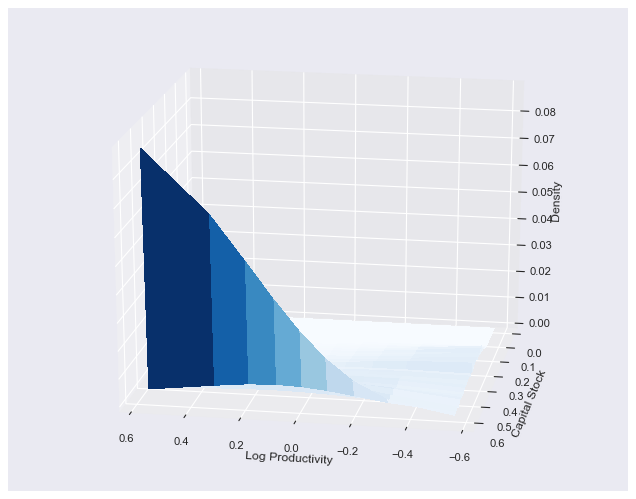
\includegraphics[width=\textwidth]{figure_std}
	\caption{Stationary Distribution of Firms}
	\label{fig:figure_std}
\end{figure}

\subsection{Policy Function}

In this subsection, I present the results of Figure \ref{fig:figure_policy}. This picture shows how $ k' $ changes with capital stock $ z $ and productivity shock $ k $.

As you can see from the picture, $ k' $ is monotonically increasing with the productivity, given any level of capital stock $ k $. More importantly, it seems that $ k' $ increases faster when the shock is low (convex) while increases slower when the shock is high (concave), especially when capital stock is high.

\begin{figure}[h]
	\centering
	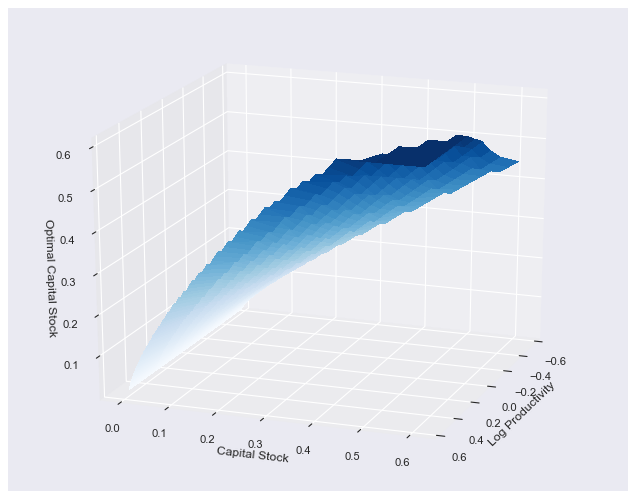
\includegraphics[width=\textwidth]{figure_policy}
	\caption{Stationary Distribution of Firms}
	\label{fig:figure_policy}
\end{figure}


\end{document}